\documentclass[t]{beamer}
\usetheme{Warsaw}
\usecolortheme{seahorse}
\usepackage{array}
\usepackage{graphicx}
\usepackage{amssymb,amsmath,mathrsfs,amsfonts}
%\usepackage[colorhighlight,display]{texpower}
%\usepackage{caption}
%\usepackage[all]{xy}
\usepackage{beamerthemesplit}
\mode<presentation>
%\usepackage{pause}
\usepackage{ulem}  % for strikethroughs
\usepackage{cancel} % for strikethroughs in math mode 
\usepackage{tikz}
\usepackage{calc}
\usetikzlibrary{shapes}
\usepackage{hyperref}
\hypersetup{pdfpagemode=FullScreen}
\usepackage{ifthen}
\usepackage{animate}
\usepackage{color}
\usepackage{type1cm}  % used for watermarking
\usepackage{eso-pic}  % used for watermarking

\usepackage[absolute,overlay]{textpos}
  \setlength{\TPHorizModule}{1mm}
  \setlength{\TPVertModule}{1mm}


\theoremstyle{plain}
\newtheorem{prop}{Proposition}
\newtheorem{thm}[prop]{Theorem}
\newtheorem{lem}[prop]{Lemma}
\newtheorem{cor}[prop]{Corollary}
\theoremstyle{definition}
\newtheorem{dfn}{Definition}
\newtheorem{rem}[prop]{Remark}
\newtheorem{ex}{Example}[section]
%\newtheorem{note}{Note}[section]
\newtheorem{exercise}{Exercise}[section]
\newcommand{\nin}{\noindent}
\newcommand{\ds}{\displaystyle}
\renewcommand{\figurename}{Figure \arabic{figure}}



\renewcommand*\familydefault{\sfdefault} 




%%%%%%%%%%%%%%%%%%%%%%%%%%5
%%%%%%%%%%%%%%%%%%%%%%%%%%%%
%%%% some commands that have different meaning in the article/presentation modes

\newcommand{\vvfill}{\mode<presentation>{\vfill}  \mode<article>{\medskip}}   %vfill in presentation only
\newcommand{\sketchspace}{ 
\mode<article>{ \medskip\noindent{\textbf{Sketch:}} \vspace*{6cm} }
\mode<presentation>{ } 
}
\newcommand{\examplespace}{ 
\mode<article>{ \medskip\noindent{\textbf{Example:}} \vspace{6cm} }
\mode<presentation>{ } 
}
\newcommand{\artsmspace}{\mode<article>{\vspace*{2cm}} }  %small space in article mode
\newcommand{\artlargespace}{\mode<article>{\vspace*{6cm}} }  %large space in article mode

\newcommand{\dx}{\,dx}

\newcommand{\soln}{{\textbf{Solution: }}\,\,\,}
\newcommand{\disp}{\displaystyle}

\newcommand{\makedate}{\vvfill
\begin{picture}(10,10)  
\put(260,-20){\mbox{\tiny{\today}}}
\end{picture}
}

\newcommand{\pd}[2]{\dfrac{\partial#1}{\partial#2}}
\newcommand{\pD}[2]{\dfrac{\partial^2#1}{\partial#2^2}}
\newcommand{\pdd}[3]{\dfrac{\partial^2#1}{\partial#2 \partial#3}}


\normalem %stops the ulem package making all the emphs into underlines...
 
 
 
 \newcommand{\refandrev}[2]{
 \begin{small}
  \hspace{6cm}
  \begin{minipage}[r]{8cm}
  Stewart,    Chapter #1   \\
  Review:  \parbox[t]{6cm}{#2}
\end{minipage}
\end{small}
}



\newcounter{heading}
\setcounter{section}{1}
\setcounter{heading}{0}

\newcommand{\makeheading}[1]{\medskip\begin{large}\noindent\textbf{{#1}}\end{large}\smallskip}

%\newenvironment{head}[1]{\medskip\stepcounter{heading}\noindent\textbf{\hspace{0.2cm}{#1}.}}{}
\newcommand{\newhead}[1]{\medskip\stepcounter{heading}\noindent\textbf{\hspace{0.2cm}{#1}.}}


\newcommand{\pf}[1]{\noindent\textit{Proof.}\vspace*{#1 cm}}
\newcommand{\sol}[1]{\noindent\textit{Solution.}\vspace*{#1 cm}}
\newcommand{\further}[1]{\begin{small}\noindent\textit{Further reading: #1}\end{small}}
\newcommand{\exr}[1]{\begin{footnotesize}\noindent\textit{\textbf{Exercises:} Stewart #1}\end{footnotesize}}


% Sets of numbers
\newcommand{\C}{\mathbb{C}}
\newcommand{\RR}{\mathbb{R}}
\newcommand{\Z}{\mathbb{Z}}
\newcommand{\N}{\mathbb{N}}
\newcommand{\Q}{\mathbb{Q}}

% Partitions
\newcommand{\PP}{\mathcal{P}}

% Limits
\newcommand{\limm}[1]{\displaystyle \lim_{x\to #1}}

% Backslash
\newcommand{\bs}{\backslash}

% functions
\newcommand{\cosec}{\mathrm{cosec}}
\newcommand{\cosech}{\mathrm{cosech}}
\newcommand{\sech}{\mathrm{sech}}
\newcommand{\Li}{\mathrm{Li}}
\newcommand{\si}{\mathrm{Si}}
\newcommand{\erf}{\mathrm{erf}}

% Domain and Range
\newcommand{\Dom}{\mathrm{Dom}}
\newcommand{\Codom}{\mathrm{Codom}}
\newcommand{\Range}{\mathrm{Ran}}



\title{Week 10:  Integration Techniques Part 2}

\begin{document}

\frame{\titlepage}

\setcounter{tocdepth}{2}
\frame{\tableofcontents
}

\AtBeginSection[]
{
\begin{frame}<beamer> 
\tableofcontents[currentsection]  % show TOC and highlight current section
\end{frame}
}



\section{Trigonometric integrals ($\tan^m{x}\sec^n{x})$}

%\begin{frame}
%\frametitle{Trigonometric integrals}
%%%%%%%%%%%%%%%%%%%%%%%%%%%%%%%%%%%%%%%%
%
%\noindent We examine integrals of the form
%\begin{enumerate}
%\item $\ds\int \sin^mx \cos^nx\,dx$
%\item $\ds\int \tan^mx \sec^nx\,dx$
%\end{enumerate}
%
%\vspace*{.5cm}
%
%\noindent There are some strategies to evaluating these integrals, but occasionally we must use some tricks and ingenuity.
%
%\noindent We begin by looking at integrals involving powers of $\sin x$ and $\cos x$.
%\end{frame}

\begin{frame}
\[ \ds\int \tan^mx \sec^nx\,dx.\] 
We consider, as above, two cases.  

\newhead{Case 1: The integral involves an even power of $\sec x$} We save one factor of $\sec^2x$ and use $\sec^2x=1+\tan^2x$ to express the remaining factors in terms of $\tan x$. Then substitute $u=\tan x$. 

\newhead{Case 2: The integral involves an odd power of $\tan x$} We save one factor of $\sec x\tan x$ and use $\tan^2x=\sec^2x-1$ to express the remaining factors in terms of $\sec x$. Then substitute $u=\sec x$. 

\medskip

\begin{itemize}
\item Recall that $\ds\int \tan{x} \,dx = \ln |\sec{x}| + C$ and $\ds\int \sec{x} \,dx = \ln |\sec{x} + \tan{x}| + C$
\end{itemize}

\end{frame}


\begin{frame}
\frametitle{Example} 

Evaluate $\ds\int\tan^6x\sec^4x\,dx$. \pause

\begin{itemize}
	\item $\ds\int\tan^6x\sec^4x\,dx = \ds\int\tan^6x\sec^2x \sec^2x \,dx = \ds\int\tan^6x (1 + \tan^2x) \sec^2x \,dx $.
	\item Let $u = \tan{x}$ and $du = \sec^2x \,dx$
	\item $\ds\int u^6 ( 1 + u^2) \, du = \ds\int u^6 + u^8 \, du $
	\item $\ds\frac{u^7}{7} + \frac{u^9}{9} + C = \frac{1}{7} \tan^7{x} + \frac{1}{9} \tan^9{x} + C$
\end{itemize}

\end{frame}

\begin{frame}
\frametitle{Example} 

Evaluate $\ds\int\tan^5x\sec^7x\,dx$. \pause

\begin{itemize}
	\item $\ds\int\tan^5x\sec^7x\,dx = \ds\int\tan^4x\sec^6x \sec x \tan x \,dx $
	\item $\ds\int(\sec^2x - 1)^2\sec^6x \sec x \tan x \,dx $.
	\item Let $u = \sec{x}$ and $du = \sec x \tan x \,dx$
	\item $\ds\int (u^2 - 1)^2 u^6 \, du = \ds\int (u^{10} - 2u^8 + u^6) \, du $
	\item $\ds\frac{u^{11}}{11} - 2\frac{u^9}{9} + \frac{u^7}{7} + C = \frac{\sec^{11}{x}}{11} - 2\frac{\sec^9{x}}{9} + \frac{\sec^7{x}}{7} + C$
\end{itemize}

\end{frame}

\begin{frame}
\frametitle{Example} 

Evaluate $\ds\int\tan^3x \,dx$. \pause

\begin{itemize}
	\item $\ds\int\tan^3x \,dx = \ds\int \tan x \tan^2x \,dx = \ds \int \tan x (\sec^2x - 1)\,dx $
	\item $\ds \int \tan x \sec^2x \,dx - \int \tan{x} \,dx $.
	\item Let $u = \tan{x}$ and $du = \sec^2x \,dx$ for the left integral
	\item $\ds\frac{\tan^{2}{x}}{2} - \ln |\sec{x}| + C$
\end{itemize}

\end{frame}

\begin{frame}
\frametitle{Example} 

\footnotesize

Evaluate $\ds\int\sec^3x \,dx$. \pause

\begin{itemize}
	\item Use integration by parts where $u = \sec{x}$, $du = \sec x \tan x \dx$, $dv = \sec^2x \,dx$, and $v = \tan {x}$,  and recall the formula $\ds\int u\, dv = uv - \int v \, du.$
	\item $\ds \int \sec^3{x} = \sec x \tan x - \int \sec x \tan^2 x \,dx $
	\item $ = \sec x \tan x - \ds\int \sec x (\sec^2 x - 1) \,dx $
	\item $ = \sec x \tan x - \ds\int \sec ^3 x \,dx+  \int \sec x \,dx $
	\item $ \ds \int \sec^3{x} + \sec ^3 x \,dx = \sec x \tan x - \int \sec ^3 x \,dx +  \int \sec x \,dx +  \int \sec ^3 x \,dx$
	\item $\frac{1}{2} (\sec x \tan x  + \ln |\sec {x} + \tan{x}|) + C$
\end{itemize}

\end{frame}

\begin{frame}
\frametitle{Exercise} 

$\ds\int\tan x\sec^3x\,dx$. %stewart 7.2 question 21
\begin{itemize}
	\item Ans: $\ds\frac{1}{3}u^3 + C = \frac{1}{3}\sec^3{x} + C$
\end{itemize}
$\ds\int\tan^3x\sec^6x\,dx$. %question 29
\begin{itemize}
	\item Ans: $\ds\frac{1}{8}\tan^8{x} + \frac{1}{3}\tan^6{x} + \frac{1}{4}\tan^4{x} + C$
\end{itemize}
$\ds\int\tan^5x\,dx$. %stewart 7.2 question 31
\begin{itemize}
	\item Ans: $\frac{1}{4}\sec^4{x} - \tan^2{x} + \ln |{\sec{x}}| + C$
\end{itemize}
$\ds\int\tan^2x\sec x\,dx$. %question 32
\begin{itemize}
	\item Ans: $\ds\frac{1}{2} (\sec x \tan x - \ln |\sec{x} + \tan{x}|)  + C$
\end{itemize}

\end{frame}


\section{Trigonometric substitution}


\begin{frame}
\frametitle{Trigonometric substitution}


\noindent We now look at integrals of the form $\int \sqrt{a^{2} - x^{2}}\,dx$, where $a>0$.  A good strategy is to change variables from $x$ to $\theta$ by using the substitution $x = a\sin\theta$.  The identity $1 - \sin^2{\theta} = \cos^2\theta$ allows us to get rid of the root sign because

$$ \sqrt{a^{2} - x^{2}} =  \sqrt{a^{2} - a^{2}\sin^2\theta} = \sqrt{a^2(1 - \sin^2\theta)} = \sqrt{a^2\cos^2\theta} = a |\cos\theta|$$

If we assume that the range $\theta$ is $[-\frac{\pi}{2},\frac{\pi}{2}]$, then it becomes $a \cos\theta$

\begin{figure}[t]
\begin{center}
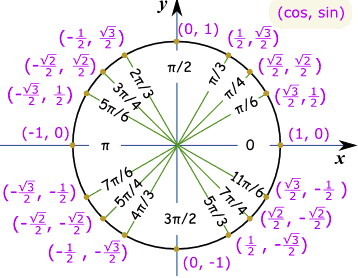
\includegraphics[scale=0.3]{fig/cos_sin}
\end{center}
\end{figure}

\end{frame}

\begin{frame}
\newhead{Table of substitutions and trigonometric functions}\\
\noindent
\begin{center}
\renewcommand{\arraystretch}{1.5}
\begin{tabular}{|c|c|c|c|}
\hline
Expression & Substitution & Range for $\theta$  & Identity \\
\hline
$\sqrt{a^2-x^2}$ & $x=a\sin\theta$ & $[-\frac{\pi}{2},\frac{\pi}{2}]$ & $1 - \sin^2\theta = \cos^2\theta$ \\
$\sqrt{a^2+x^2}$ & $x=a\tan\theta$ & $(-\frac{\pi}{2},\frac{\pi}{2})$  & $1 + \tan^2\theta = \sec^2\theta$\\
$\sqrt{x^2-a^2}$ & $x=a\sec\theta$ & $[0,\frac{\pi}{2})\cup[\pi,\frac{3\pi}{2})$ & $ \sec^2\theta - 1 = \tan^2\theta$ \\
\hline
\end{tabular}
\end{center}

\begin{center}
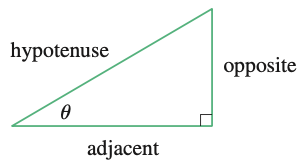
\includegraphics[scale=0.3]{fig/hypothenus}
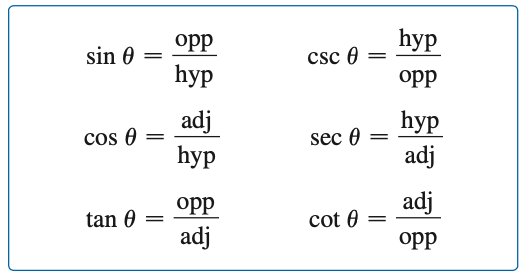
\includegraphics[scale=0.3]{fig/hypothenus2}
\end{center}

\end{frame}

\begin{frame}
\footnotesize
\frametitle{Example}
Evaluate $\displaystyle\int\frac{\sqrt{9-x^{2}}}{x^{2}}\,dx.$ \pause

\medskip

Let $x = 3 \sin \theta$,  then $dx = 3 \cos\theta d\theta$, hence $\sqrt{9 - x^2} = \sqrt{9 - 9 \sin^2\theta} = \sqrt{9 (1 - \sin^2\theta)} = \sqrt{9\cos^2\theta} = 3 |\cos\theta| = 3 \cos\theta$

\begin{align*}
\displaystyle\int\frac{\sqrt{9-x^{2}}}{x^{2}}\,dx &= \displaystyle\int \frac{3 \cos\theta}{9 \sin^2\theta}3\cos\theta d\theta\\
&=\displaystyle\int \frac{\cos^2\theta}{\sin^2\theta}d\theta = \int \cot^2\theta d\theta\\
&=\displaystyle\int(\csc^2\theta -1)d\theta = -\cot\theta - \theta + C
\end{align*}

See figure 1, we know that $\cot\theta =\frac{\sqrt{9 - x^2}}{x}$,  we also know that $\theta = sin^{-1}(\frac{x}{3})$ thus

$$\displaystyle\int\frac{\sqrt{9-x^{2}}}{x^{2}}\,dx. = -\frac{\sqrt{9 - x^2}}{x} - sin^{-1}(\frac{x}{3}) + C$$

\begin{textblock}{0.3}(100,0)
      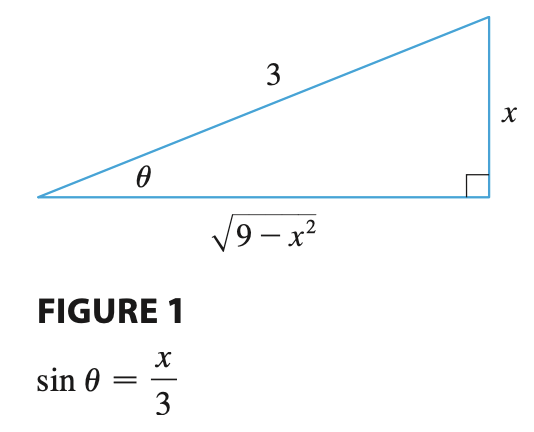
\includegraphics[scale=0.3]{fig/cot}
\end{textblock}

\end{frame}

\begin{frame}
\footnotesize
\frametitle{Example}
Find the area enclosed by the ellipse $\frac{x^2}{a^2}+\frac{y^2}{b^2}=1$ \pause

\begin{itemize}
	\item $\frac{y^2}{b^2} = 1 - \frac{x^2}{a^2} = \frac{a^2 - x^2}{a^2}$ or
	\item $y = \pm \frac{b}{a}\sqrt{a^2 - x^2}$
\end{itemize}

Because the ellipse is symmetric with respect to both axes,  the total area A is four times the area in the first quadrant (see Figure 2). The part of the ellipse in the first quadrant is given by the function

$$y = \frac{b}{a}\sqrt{a^2 - x^2}  \text{   where   }  0 \leq x \leq a \text{    thus    }$$
$$\frac{1}{4}A = \int_0^a\frac{b}{a}\sqrt{a^2 - x^2} \,dx$$

Let $x = a\sin\theta$, then $\dx = a\cos\theta d\theta$.  To change the limits of integration, when $x=0$, $a \sin\theta = 0$,  so $\theta = 0$.  When $x=a$, $a\sin\theta = a$, thus $\theta = \frac{\pi}{2}$.  

\medskip  

\textit{(continued next slide)}

\begin{textblock}{0.3}(100,0)
      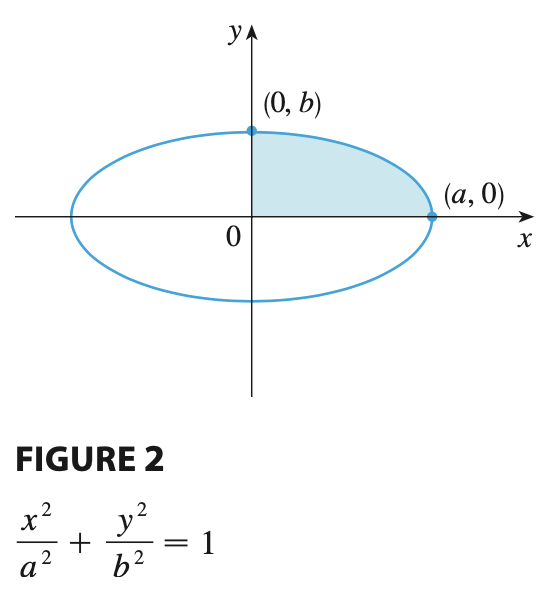
\includegraphics[scale=0.3]{fig/eclipse}
\end{textblock}

\end{frame}

\begin{frame}

\newhead{Continued..}

\begin{align*}
A &= 4\frac{b}{a}\int_0^a \sqrt{a^2 - x^2} \,dx = 4\frac{b}{a}\int_0^{\pi/2} a \cos\theta \cdot a\cos\theta d\theta\\
&= 4ab \int_0^{\pi/2} \cos^2\theta d\theta = 4ab\int_0^{\pi/2}\frac{1}{2}(1 + \cos 2\theta) d\theta\\
&= 2ab \left[\theta + \frac{1}{2}\sin 2\theta\right]_0^{\pi/2} = 2ab\left(\frac{\pi}{2} + 0 - 0\right)\\
&= \pi a b
\end{align*}

\end{frame}

\begin{frame}

\frametitle{Example} 
\footnotesize
Find $\int \frac{1}{x^{2}\sqrt{x^{2}+4}}\,dx$. \pause

\medskip

Let $x = 2\tan\theta$, then $dx = 2 \sec^2\theta d\theta$, thus

$$\sqrt{x^2 + 4} = \sqrt{4(\tan^2\theta + 1)} = \sqrt{4\sec^2\theta} = 2 |\sec\theta| = 2 \sec\theta$$

So we have

$$\int\frac{dx}{x^2\sqrt{x^2 + 4}} = \int\frac{2sec^2\theta d\theta}{4\tan^2\theta \cdot 2\sec\theta} = \frac{1}{4}\int\frac{sec\theta}{\tan^2\theta}d\theta$$

We put everything in terms of $\sin\theta$ and $\cos\theta$:

$$\frac{\sec\theta}{\tan^2\theta} = \frac{1}{\cos\theta} \cdot \frac{\cos^2\theta}{\sin^2\theta} = \frac{\cos\theta}{\sin^2\theta}$$

\textit{(continued next slide)}

\begin{textblock}{0.3}(100,0)
      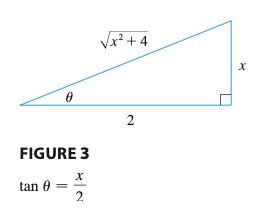
\includegraphics[scale=0.6]{fig/csc}
\end{textblock}

\end{frame}

\begin{frame}

\newhead{Continued...}

Here make the substitution $u = \sin\theta$, we have

\begin{align*}
\int \frac{dx}{x^2\sqrt{x^2 + 4}} &= \frac{1}{4}\int \frac{cos\theta}{sin^2\theta} d\theta = \frac{1}{4}\int \frac{du}{u^2}\\
&= \frac{1}{4} \left(-\frac{1}{u}\right) + C = -\frac{1}{4\sin\theta} + C\\
&= -\frac{csc\theta}{4} + C
\end{align*}

Using figure 3, we determine that $\csc\theta = \frac{\sqrt{x^2 + 4}}{x}$, so

$$\frac{dx}{x^2\sqrt{x^2 + 4}} = -\frac{\sqrt{x^2 + 4}}{4x} + C$$

\begin{textblock}{0.3}(100,0)
      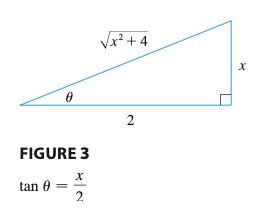
\includegraphics[scale=0.6]{fig/csc}
\end{textblock}


\end{frame}



\begin{frame}

\frametitle{Example} 

Find $\int\frac{x}{\sqrt{x^{2}+4}}\,dx$. \pause

\medskip

It would be possible to use the trigonometric substitution $x = 2\tan\theta$ here.  But the direct substitution $u = x^2 + 4$ is simpler, because then $du = 2x\dx$ and

$$\int\frac{x}{\sqrt{x^2 + 4}}dx = \frac{1}{2}\int\frac{du}{\sqrt{u}} = \sqrt{u} + C = \sqrt{x^2 + 4} + C$$

Thus, note that even when trigonometric substitutions are possible, they may not give the easiest solution.

\end{frame}

\begin{frame}
\frametitle{Exercise}

\begin{itemize}
	\item $\int_0^3 \frac{x}{\sqrt{36 - x^2}}$ %Stewart chapter 7.3 No. 6
	\begin{itemize}
		\item Ans: $6 - 3\sqrt{3}$
	\end{itemize}
	\item $\int \frac{\sqrt{1 + x^2}}{x}$ %Stewart chapter 7.3 No. 19
	\begin{itemize}
		\item Ans: $\ln|\frac{\sqrt{1 + x^2} - 1}{x}| + \sqrt{1 + x^2} + C$
	\end{itemize}
	\item  $\int\frac{1}{\sqrt{x^{2} - a^{2}}}\,dx$, where $a>0$ 
	\begin{itemize}
		\item Ans: $\ln|x + \sqrt{x^2 - a^2}| - \ln{a} + C$ %Example 5 Stewart chapter 7.3
	\end{itemize}
\end{itemize}

\end{frame}



\end{document}
